\documentclass[12pt,a4paper]{article}

\renewcommand*\contentsname{Sadržaj}
\renewcommand{\figurename}{Slika}
\renewcommand{\tablename}{Tabela}
\renewcommand\refname{Reference}
\renewcommand{\arraystretch}{1.25}

\usepackage[margin=0.85in]{geometry}
\usepackage{graphicx}
\usepackage{float}
\usepackage{listings}
\usepackage{multirow}
\usepackage[table]{xcolor}
\usepackage{colortbl}
\usepackage{color}
\usepackage{hyperref}
\usepackage{ctable}
\usepackage{array}
\usepackage{hhline}
\usepackage{caption}
\usepackage{amsfonts}
\usepackage{flowchart}
\usepackage{algpseudocode}
\usepackage[shortlabels]{enumitem}
\usepackage{algorithm2e}
\renewcommand{\algorithmcfname}{Algoritam}
\usetikzlibrary{arrows}

\lstloadlanguages{C,C++,csh,Java}

\definecolor{red}{rgb}{0.6,0,0} 
\definecolor{blue}{rgb}{0,0,0.6}
\definecolor{green}{rgb}{0,0.8,0}
\definecolor{cyan}{rgb}{0.0,0.6,0.6}
\definecolor{magnolia}{rgb}{0.97, 0.96, 1.0}
\definecolor{colora}{rgb}{0.67, 0.8, 0.94}
\definecolor{colorb}{rgb}{0.67, 0.94, 0.82}
\definecolor{colord}{rgb}{0.67, 0.9, 0.93}
\definecolor{colore}{rgb}{0.6, 0.73, 0.89}
\definecolor{colorf}{rgb}{0.61, 0.87, 1.0}
\definecolor{grey}{rgb}{0.75, 0.75, 0.75}

\lstset{
language=csh,
basicstyle=\footnotesize\ttfamily,
numbers=left,
numberstyle=\tiny,
numbersep=5pt,
tabsize=2,
extendedchars=true,
breaklines=true,
frame=b,
stringstyle=\color{blue}\ttfamily,
showspaces=false,
showtabs=false,
xleftmargin=17pt,
framexleftmargin=17pt,
framexrightmargin=5pt,
framexbottommargin=4pt,
commentstyle=\color{green},
morecomment=[l]{//}, %use comment-line-style!
morecomment=[s]{/*}{*/}, %for multiline comments
showstringspaces=false,
morekeywords={ abstract, event, new, struct,
as, explicit, null, switch,
base, extern, object, this,
bool, false, operator, throw,
break, finally, out, true,
byte, fixed, override, try,
case, float, params, typeof,
catch, for, private, uint,
char, foreach, protected, ulong,
checked, goto, public, unchecked,
class, if, readonly, unsafe,
const, implicit, ref, ushort,
continue, in, return, using,
decimal, int, sbyte, virtual,
default, interface, sealed, volatile,
delegate, internal, short, void,
do, is, sizeof, while,
double, lock, stackalloc,
else, long, static,
enum, namespace, string},
keywordstyle=\color{cyan},
identifierstyle=\color{red},
backgroundcolor=\color{magnolia},
}

\DeclareCaptionFont{white}{\color{white}}
\DeclareCaptionFormat{listing}{\colorbox{blue}{\parbox{\textwidth}{\hspace{15pt}#1#2#3}}}
\captionsetup[lstlisting]{format=listing,labelfont=white,textfont=white, singlelinecheck=false, margin=0pt, font={bf,footnotesize}}

\newcolumntype{a}{>{\columncolor{colora}}c}
\newcolumntype{b}{>{\columncolor{colorb}}c}
\newcolumntype{d}{>{\columncolor{colord}}c}
\newcolumntype{e}{>{\columncolor{colore}}c}
\newcolumntype{f}{>{\columncolor{colorf}}c}
\newcolumntype{P}[1]{>{\centering\arraybackslash}p{#1}}
\newcolumntype{?}{!{\vrule width 1pt}}

\begin{document}

\begin{titlepage}
	\centering
	{\scshape Univerzitet u Sarajevu \par}
	{\scshape Elektrotehnički Fakultet \par}
	{\scshape Odsjek za Računarstvo i Informatiku \par}
	\vspace{2cm}
	{\Large\scshape Biomedicinski Signali i Sistemi\par}
	\vspace{2.5cm}
	{\huge\bfseries Seminarski Rad\par}
	\vspace{2.5cm}
	{\huge\bfseries Aritmija i hipertenzija te njihov utjecaj na EKG signale\par}
	\vspace{2.5cm}
	\Large Student: \par
	{\Large\itshape \textsc{Krupalija} Ehlimana, 1431/17461\par}
	\vfill
	Predmetni nastavnik:\par
	v. prof. dr. \textsc{Dušanka Bošković}, dipl. ing. el.
	\vfill
	{\large Juli, 2019\par}
\end{titlepage}

\pagenumbering{gobble}

\tableofcontents

\newpage

\pagenumbering{arabic}

\section{Uvod}

\quad Elektrokardiogram (EKG) je graf koji prikazuje promjenu u električnoj aktivnosti srca kroz vrijeme. Korištenjem ove tehnologije moguće je analizirati rad srca, budući da tokom različitih faza rada srca (sistole i dijastole) dolazi do pojave različitih vrijednosti napona koje je moguće izmjeriti te na taj način detektovati karakteristike rada srca (tzv. PQRS kompleks prikazuje se na EKG signalu te je njegovom analizom moguće doći do velikog broja podataka koji mogu biti korisni u detektovanju simptoma te dijagnostici različitih stanja i bolesti). \\

Jedan veoma čest i rasprostranjen poremećaj srca je aritmija, te je vršenje dijagnosticiranja ovog poremećaja jednostavno i brzo, budući da se na jednom EKG signalu može vrlo lako uočiti nepravilnost u radu srca. Jedan veoma čest poremećaj usko vezan s radom srca je visok krvni pritisak, koji u različitim slučajevima može dovesti do različitih poremećaja u radu srca, koje je također veoma lako uočiti na EKG signalu. Budući da je vršenje elektrokardiografije bezbolno i brzo, korištenje ove tehnike za dijagnosticiranje i analizu veoma je često. \\

Pojava velikog broja softverskih alata za prikupljanje i analizu EKG signala olakšava analizu svih ovih podataka. Postoji veliki broj baza podataka u kojima se nalaze sortirani EKG signali pacijenata s različitim poremećajima, među kojima važno mjesto zauzimaju baze podataka pacijenata koji imaju aritmiju i hipertenziju (visok krvni pritisak). Iz tog razloga, analizom ovakvih EKG signala moguće je doći do velikog broja informacija koje mogu pomoći pri dijagnosticiranju ovih bolesti veoma rano nakon njihovog nastanka kako bi se mogle tretirati i uspješno kontrolisati (te i izliječiti). \\

U ovom radu biti će dat opis aritmije i visokog krvnog pritiska kao poremećaja koji se mogu dovesti u vezu s EKG signalima, te će biti izvršena analiza signala iz baza podataka pacijenata s ovim poremećajima koristeći alate razvijene u programskom jeziku \textit{Python}, nakon čega će se ova dva poremećaja pokušati dovesti u vezu te se donijeti zaključci o zajedničkim osobinama EKG signala iz ovih baza podataka.

\newpage

\section{Poremećaj ritma rada srca}

\quad Normalan rad srca karakteriše stabilan ritam rada - srce koje pravilno radi, pumpa krv u pravilnim vremenskim razmacima te je ritam srca pravilan i ujednačen. U slučaju pravilnog rada srca, na EKG snimku moguće je vidjeti pravilan razmak između PQRS kompleksa - depolarizacija pretkomora i komora, grčenje srčanog mišića, pumpanje krvi te polarizacija i opuštanje srčanog mišića dešavaju se u pravilnim vremenskim razmacima. Ovi vremenski razmaci mogu varirati u rasponu od maksimalno $\delta$ = 0.16 sekundi. EKG snimak pacijenata koji nemaju aritmiju sastoji se od 60 do 100 PQRS kompleksa po minuti (mada se granica tolerancije u nekim slučajevima može spustiti i do 50 bpm). \cite{arrhythmia-book} \\

Tipičan EKG snimak pacijenta čije srce karakteriše pravilan rad moguće je vidjeti na Slici \ref{s1}. Vidljivo je da se otkucaji srca javljaju u pravilnim razmacima, bez većih fluktuacija koje bi ukazivale na neku bolest poput aritmije.

\begin{figure}[H]
\center
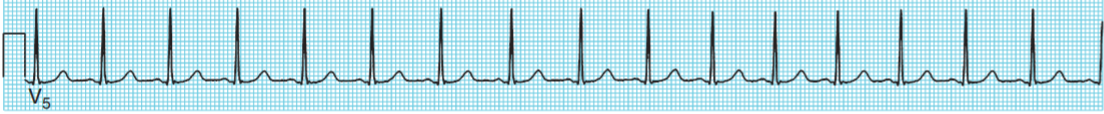
\includegraphics[scale=0.7]{../res/s1.PNG}
\caption{Prikaz EKG signala pacijenta koji nema srčanih problema}
\label{s1}
\end{figure}

Ukoliko srce pacijenta kuca sporije od 60 (odnosno 50), ili brže od 100 puta u minuti, te ukoliko su varijacije između srednje veličine razmaka između pojedinačnih otkucaja (PQRS kompleksa) veće od 0.16 sekundi, pacijentu se dijagnosticira stanje koje se naziva \textbf{aritmija}. Aritmija zapravo označava zdravstveno stanje u kojem srce nije u mogućnosti da ispravno kontroliše svoj rad, te se kao posljedica faze kontrakcija i opuštanja dešavaju u nepravilnim razmacima, te ih zbog toga ima ili manje, ili više nego što bi trebalo kako bi srčani sistem ispravno funkcionisao, te kako bi količina krvi u krvotoku bila u dozvoljenim granicama. \cite{arrhythmia-basics} \\ 

Tipičan EKG snimak pacijenta čije srce karakteriše nepravilan rad moguće je vidjeti na Slici \ref{s2}. Vidljivo je da se otkucaji srca javljaju u izrazito nepravilnim razmacima, s velikim fluktuacijama koje nedvosmisleno vode do zaključka da pacijent boluje od aritmije.

\begin{figure}[H]
\center
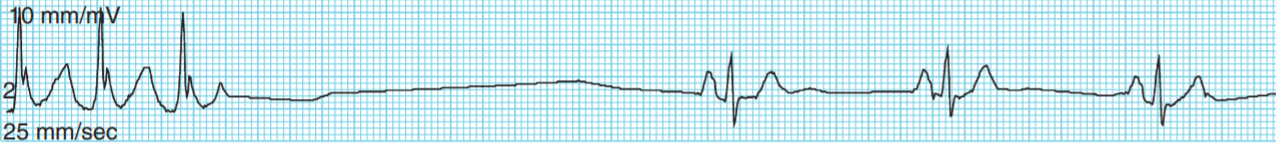
\includegraphics[scale=0.6]{../res/s2.PNG}
\caption{Prikaz EKG signala pacijenta koji boluje od aritmije}
\label{s2}
\end{figure}

\quad Postoje dva glavna uzroka aritmije:

\begin{enumerate}

\item \textit{Nepravilan rad sinusnog čvora}, tzv. \textit{pacemaker}-a srca, zbog kojeg srce nepravilno pumpa krv te se depolarizacija ne dešava uvijek u isto vrijeme, već u nepravilnim razmacima. Ovakav tip aritmije naziva se \textbf{sinusnom aritmijom}, te je karakterističan za sportiste, čiji metabolizam i način života dovode do poremećaja u funkcijama sinusnog čvora, zbog čega se javlja nepravilan rad srca. Tipičan primjer ovog tipa aritmije može se vidjeti na Slici \ref{s3}.

\begin{figure}[H]
\center
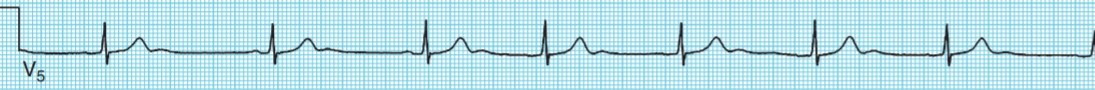
\includegraphics[scale=0.7]{../res/s3.PNG}
\caption{Prikaz EKG signala pacijenta koji boluje od sinusne aritmije}
\label{s3}
\end{figure}

\item \textit{Nepravilna električna provodnost}, koja se odnosi na nakupljanje električnog naboja koji dovodi do pojave lažne depolarizacije samo trenutak nakon što se završi jedan ciklus rada srca (otkucaj), što za posljedicu ima novi ciklus (novi otkucaj) prije nego prođe faza mirovanja. Ovakav tip aritmije karakterističan je za pacijente koji koriste opojna sredstva ili neku drugu vrstu stimulanata što dovodi do poremećaja u električni sredini cijelog tijela, te što za posljedicu ima i poremećaj rada srca. Tipičan primjer ovog tipa aritmije može se vidjeti na Slici \ref{s4}.

\begin{figure}[H]
\center
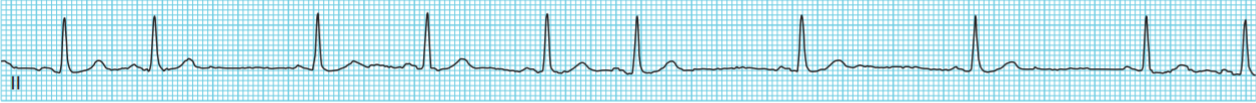
\includegraphics[scale=0.6]{../res/s4.PNG}
\caption{Prikaz EKG signala pacijenta koji boluje od ventrikularne aritmije}
\label{s4}
\end{figure}

\end{enumerate}

\newpage

\section{Poremećaji krvnog pritiska}

\quad Vrijednost krvnog pritiska u arterijama stalno se mijenja, jer krv nije statična komponenta u tijelu, već konstantno protiče kroz krvne žile (prosječan protok krvi kroz arterije mjeri se u kubnim centimetrima i ovisi od veličine arterije i njenog položaja u tijelu). \cite{blood-pressure}
Postoje dvije karakteristične vrijednosti krvnog pritiska:

\begin{enumerate}

\item \textit{Sistolni krvni pritisak}, koji predstavlja maksimalnu vrijednost krvnog pritiska koja se pojavljuje u fazi kontrakcije srca (tokom sistole);

\item \textit{Dijastolni krvni pritisak}, koji predstavlja minimalnu vrijednost krvnog pritiska koja se pojavljuje u fazi opuštanja srca (tokom dijastole).

\end{enumerate}

Normalan krvni pritisak iznosi oko 120 mmHg (sistolni krvni pritisak) i 80 mmHg (dijastolni krvni pritisak), što se jednostavnije označava kao 120/80. Postoji više vrsta poremećaja krvnog pritiska, poput npr. malog raspona između sistolnog i dijastolnog pritiska (što može simptom velikog broja stanja, od nesvjestice do problema s radom srca), širokog raspona pulsa (što može biti simptom problema u radu aorte ili drugih arterija u tijelu) i sl. \cite{wide-pulse-pressure} \\

Dva najčešća poremećaja krvnog pritiska su \textbf{hipotenzija} (nizak krvni pritisak) i \textbf{hipertenzija} (visok krvni pritisak). Niskim, odnosno visokim krvnim pritiskom smatraju se sve vrijednosti krvnog pritiska koje su manje ili jednake, odnosno veće ili jednake tipičnim vrijednostima (npr. visokim krvnim pritiskom smatra se i krvni pritisak 140/110 i 130/80, pri čemu u prvom slučaju postoji poremećaj uskog raspona pulsa, dok u drugom slučaju postoji poremećaj širokog raspona pulsa). Glavna razlika između ova dva poremećaja, kada su u pitanju analize EKG signale, predstavljaju posljedice ovih stanja na rad srca. \\

U slučaju niskog krvnog pritiska, može doći do nesvjestice te težih problema koji mogu biti opasni po život, no nizak krvni pritisak ne može biti uzrok oštećenja srca niti srčanih funkcija - naprotiv, nizak krvni pritisak je često simptom disfunkcije srca (odnosno, srce koje slabije radi uzrokuje slabiji protok krvi kroz arterije, te je samim tim i krvni pritisak niži) \cite{low-pressure}. S druge strane, loše ili nikakvo tretiranje visokog krvnog pritiska može dovesti do oštećenja ne samo funkcija arterija, već i kompletnog srca. Iz tog razloga mnogo je važnije vršiti analizu EKG signala kod pacijenata s visokim krvnim pritiskom kako bi se utvrdilo da li ima poremećaja u ritmu rada srca, dok su EKG signali pacijenata s niskim krvnim pritiskom karakterisani manjim amplitudama, no bez tendencije promjena u samim fazama rada srca kroz vrijeme. \cite{high-pressure} \\

Na Slici \ref{s5} prikazan je EKG signal pacijenta koji duži vremenski period boluje od visokog krvnog pritiska, bez korištenja lijekova za kontrolisanje ovog stanja. Na slici je vidljivo da je na samom grafu veoma teško utvrditi ikakvu pravilnost u ritmu rada srca, da PQRS kompleksi imaju različite oblike u svakom ciklusu rada srca (odnosno, da grčenje i opuštanje srca imaju različita trajanja i intenzitete), na osnovu čega je veoma lako zaključiti da visok krvni pritisak nije stanje koje se ne bi trebalo tretirati, jer može dovesti do velikog broja poremećaja srca, kao i drugih dijelova organizma. \cite{pressure-ECG}

\begin{figure}[H]
\center
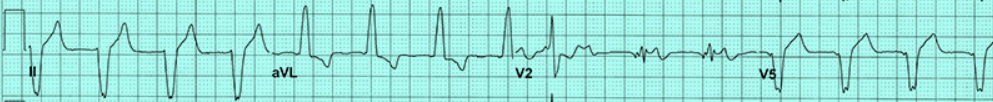
\includegraphics[scale=0.7]{../res/s5.PNG}
\caption{Prikaz EKG signala pacijenta koji boluje od hipertenzije \cite{pressure-ECG}}
\label{s5}
\end{figure}

\newpage

\section{Analiza EKG signala}

\quad Za analizu EKG signala pacijenata s prethodno opisanim vrstama poremećaja (aritmija i visok krvni pritisak) biti će korištene sljedeće PhysioNet baze podataka \cite{physionet}:

\begin{itemize}
\renewcommand\labelitemi{-}

\item \textit{Baza podataka za pacijente s aritmijom}: \href{https://physionet.org/physiobank/database/mitdb/}{MIT-BIH Arrhythmia Database} \cite{mit-bih};

\item \textit{Baza podataka za pacijente s visokim krvnim pritiskom}: \href{https://physionet.org/physiobank/database/shareedb/}{Smart Health for Assessing the Risk of Events via ECG (SHAREE) Database} \cite{sharee}.

\end{itemize}

\newpage

\bibliographystyle{IEEEtran}
\bibliography{bibliography}

\end{document}